\documentclass[10pt,a4paper,oneside]{report}

%====================== PACKAGES ======================

%police et mise en page (marges) du document
\usepackage[T1]{fontenc}
\usepackage[hmargin=2.5cm,vmargin=2cm]{geometry}
\usepackage[french]{babel}
\usepackage[utf8]{inputenc}
%pour gérer les positionnement d'images
\usepackage{float}
\usepackage{amsmath}
\usepackage{graphicx}
\usepackage{xcolor}
\graphicspath{{img/}}
%\usepackage[colorinlistoftodos]{todonotes}
\usepackage{url}
%pour les informations sur un document compilé en PDF et les liens externes / internes
\usepackage{hyperref}
%pour la mise en page des tableaux
\usepackage{array}
\usepackage{tabularx}
\usepackage{subcaption}
%pour utiliser \floatbarrier
%\usepackage{placeins}
%\usepackage{floatrow}
%espacement entre les lignes
\usepackage{setspace}
% pour les codes
\usepackage{listings}
\lstset{
  aboveskip=3mm,
  belowskip=-2mm,
  basicstyle=\footnotesize,
  breakatwhitespace=false,
  breaklines=true,
  captionpos=b,
  commentstyle=\color{red},
  deletekeywords={...},
  escapeinside={\%*}{*)},
  extendedchars=true,
  framexleftmargin=16pt,
  framextopmargin=3pt,
  framexbottommargin=6pt,
  frame=tb,
  keepspaces=true,
  keywordstyle=\color{blue},
  language=C,
  literate=
  {²}{{\textsuperscript{2}}}1
  {⁴}{{\textsuperscript{4}}}1
  {⁶}{{\textsuperscript{6}}}1
  {⁸}{{\textsuperscript{8}}}1
  {€}{{\euro{}}}1
  {é}{{\'e}}1
  {è}{{\`{e}}}1
  {ê}{{\^{e}}}1
  {ë}{{\¨{e}}}1
  {É}{{\'{E}}}1
  {Ê}{{\^{E}}}1
  {û}{{\^{u}}}1
  {ù}{{\`{u}}}1
  {â}{{\^{a}}}1
  {à}{{\`{a}}}1
  {á}{{\'{a}}}1
  {ã}{{\~{a}}}1
  {Á}{{\'{A}}}1
  {Â}{{\^{A}}}1
  {Ã}{{\~{A}}}1
  {ç}{{\c{c}}}1
  {Ç}{{\c{C}}}1
  {õ}{{\~{o}}}1
  {ó}{{\'{o}}}1
  {ô}{{\^{o}}}1
  {Õ}{{\~{O}}}1
  {Ó}{{\'{O}}}1
  {Ô}{{\^{O}}}1
  {î}{{\^{i}}}1
  {Î}{{\^{I}}}1
  {í}{{\'{i}}}1
  {Í}{{\~{Í}}}1,
  morekeywords={*,...},
  numbers=left,
  numbersep=10pt,
  numberstyle=\tiny\color{black},
  rulecolor=\color{black},
  showspaces=false,
  showstringspaces=false,
  showtabs=false,
  stepnumber=1,
  stringstyle=\color{gray},
  tabsize=4,
  title=\lstname,
}

%====================== INFORMATION ET REGLES ======================

%rajouter les numérotation pour les \paragraphe et \subparagraphe
\setcounter{secnumdepth}{4}
\setcounter{tocdepth}{4}

\hypersetup{							% Information sur le document
pdfauthor = {Vovard Marine,
            Dupoux Mathieu},			% Auteurs
pdftitle = {Sandwich -
			Implémentation d'un automate cellulaire en language C},			% Titre du document
pdfsubject = {Mémoire de Projet},		% Sujet
pdfkeywords = {Tag1, Tag2, Tag3, ...},	% Mots-clefs
pdfstartview={FitH}}					% ajuste la page à la largueur de l'écran
%pdfcreator = {MikTeX},% Logiciel qui a crée le document
%pdfproducer = {}} % Société avec produit le logiciel

\newcommand{\hsp}{\hspace{20pt}}
\newcommand{\HRule}{\rule{\linewidth}{0.5mm}}
\setlength{\parskip}{0.5em}
\definecolor{gray75}{gray}{0.75}
\makeatletter
\def\@makechapterhead#1{%
  {\parindent \z@ \Huge\bfseries
      \interlinepenalty\@M
      \thechapter\hsp\textcolor{gray75}{|}\hsp \Huge\bfseries #1 \hfill
      \vskip -15pt
      \HRule
      \vskip 15pt
  }}
\makeatother

\renewcommand{\familydefault}{\sfdefault}
\usepackage{lmodern}

%======================== DEBUT DU DOCUMENT =========================

\begin{document}
\begin{titlepage}
\begin{center}

% Upper part of the page. The '~' is needed because only works if a paragraph has started.

\includegraphics[width=0.5\textwidth]{./logo}~\\[1cm]

% Title
\HRule \\[0.4cm]

{\Huge \bfseries Rapport de projets Informatique S5\\
Sandwich \\[0.4cm] }
{\Large \bfseries Rapport complet \\[0.4cm] }

\HRule \\[1.5cm]

% Author and supervisor
\begin{minipage}{0.4\textwidth}
\begin{flushleft} \large
\emph{Auteurs:} Marine \textsc{Vovard}\\
\phantom{\emph{Auteurs:} }Mathieu \textsc{Dupoux}\\
\end{flushleft}
\end{minipage}
\begin{minipage}{0.5\textwidth}
\begin{flushright} \large
\emph{Responsable de projet}:
David \textsc{Renault}\\
\emph{Enseignant référent}:
Michaël \textsc{Clément}
\end{flushright}
\end{minipage}

\vfill

% Bottom of the page
{\large \today}

\end{center}
\end{titlepage}
\tableofcontents
\thispagestyle{empty}

\cleardoublepage

%====================== INCLUSION DES PARTIES =======================

\chapter{Vue globale du projet}
\section{Énoncé et objectif du sujet}

Ce rapport repose sur l'implémentation d'un automate cellulaire - une grille régulière de cellules contenant chacune un état choisi parmi un ensemble fini et qui peut évoluer au cours du temps\footnote{\url{https://fr.wikipedia.org/wiki/Automate_cellulaire}} - en langage C. L'un des premiers objectifs a été d'implémenter le jeu de la vie \footnote{\url{https://fr.wikipedia.org/wiki/Jeu_de_la_vie}} de John Cownway. La suite du projet nous a conduit a ajouter de nouvelles fonctionnalités ainsi qu'à optimiser les performances de notre programme initial. L'énoncé nous a guidé pour répartir ce projet en trois sections distinctes : l'implémentation des règles, celle du monde et de la file. Tous ces aspects ont alors été regroupés dans un fichier principal et des tests ont été effectué afin de vérifier le bon fonctionnement de notre algorithme. En ajoutant des fonctionnalités telles que le déplacement d'une cellule, le changement aléatoire d'état et la gestion des conflits, nous avons finalement généré deux exemples d'utilisation de notre algorithme : le jeu de la vie en couleur et la chute d'un tas de sable.

\section{Stratégie globale d'implémentation}

Le projet a débuté avec quelques règles simples:
\begin{enumerate}
    \item Les deux fichiers d'en-tête concernant les règles et le monde donnés par le sujet ne peuvent pas être modifiés ;
    \item Les données de sortie doivent être compatible avec la librairie \texttt{SDL} ;
    \item Des options peuvent être ajoutées à l'exécutable pour laisser la possibilité à l'utilisateur de modifier la taille du monde et sa génération aléatoire.
    \item L'utilisation de la compilation séparée et l'utilisation d'un \texttt{Makefile} est obligatoire.
\end{enumerate}

Suite à ces exigences, nous nous sommes appuyés sur trois structures principales: le monde qui est une image 2D remplie de pixels, les règles qui déterminent le comportement de l'automate et la file qui stocke les changements à appliquer sur le monde une fois toutes les cellules étudiées.

Le programme principal fonctionne de la manière suivante :
\begin{itemize}
    \item Dans un premier temps, nous créons un monde soit aléatoire, soit définit dans le code ;
    \item On ajoute les règles créées dans le fichier \texttt{rule.c} et stockées dans un tableau présent dans ce même fichier ;
    \item Pour chaque image à générer :
    \begin{itemize}
        \item On parcourt toutes les cellules et on regarde si elles sont compatibles avec une règle. Si c'est le cas, on choisit quel changement effectuer (un changement d'état ou un déplacement) ;
        \item On ajoute ces changements à une file ;
        \item On défile tous les changements et on les applique sur le monde en résolvant les conflits possibles lors des déplacements d'une cellule. Le choix du gagnant est fait aléatoirement.
    \end{itemize}
\end{itemize}     
\vspace{\parskip}

Les tests ont été effectués de manière à ce que chaque grande partie de notre algorithme soit vérifiée. Il existe donc des tests qui vérifient l'implémentation du monde et de ses fonctions, l'implémentation des règles et ses applications, et l'implémentation des files. Finalement, un test a été ajouté à la suite  d'un ajout d'une fonctionnalité du programme : la gestion des conflits.

\section{Organisation et dépendances du projet}

Notre répertoire de travail est composé de trois dossiers:
\begin{itemize}
    \item \texttt{src/} (source) : on y trouve tous les fichiers .c et .h nécessaires à la compilation du programme principal; \texttt{project.c} (cf \ref{fig:GrapheDepSource})
    \item \texttt{tst/} (tests) : on y répertorie les fichiers nécessaires aux tests des fonctions créées dans le dossier \texttt{src/} (cf \ref{fig:GrapheDepTests});
    \item \texttt{doc/} (documents) : on y stocke tous les documents nécessaires à la compilation du rapport du projet;
\end{itemize}

En racine du projet, seuls sont présents le fichier Makefile ainsi que le fichier \texttt{.gitignore} et le fichier \texttt{README.md} sont dans le répertoire principal.

Il a été choisi dans ce projet de séparer de manière consciencieuse les différents domaines du programme, le but étant de faciliter la modification partielle de l'algorithme tout en gardant un programme principal fonctionnel. Deux en-têtes \texttt{rule\_ext.h} et \texttt{world\_ext.h} ont été ajoutés (respectivement pour \texttt{rule.h} et \texttt{world.h}) afin d'étendre les accès aux fonctionnalités concernés, notamment pour les programmes de tests. L'ajout de la gestion des conflits et de la file à nécessité la création de fichiers dédiés à ces aspects particuliers du programme. Finalement, des fonctions ou des structures utiles dans plusieurs fichiers mais n'appartenant à aucun domaine particulier ont été regroupés dans les fichiers \texttt{utils.c} et \texttt{utils.h}. 
\medskip


\begin{figure}[h!]
    \centering
    \begin{subfigure}{0.8\textwidth}
        \centering
        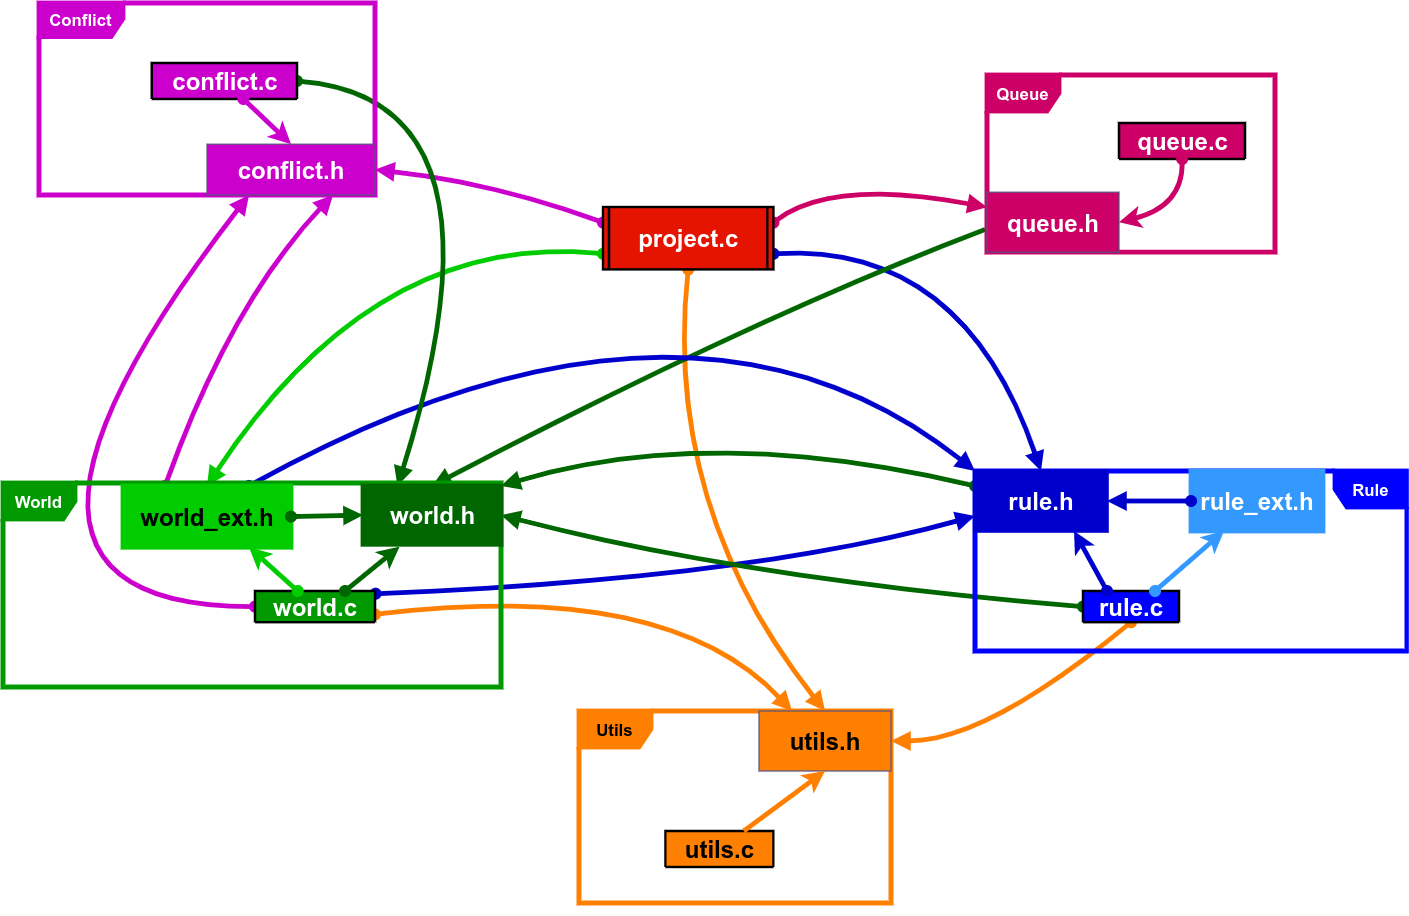
\includegraphics[width=\textwidth]{src.png}
        \caption{Dépendances des sources}
        \label{fig:GrapheDepSource}
    \end{subfigure}
    
    \bigskip
    
    \begin{subfigure}{0.8\textwidth}
        \centering
        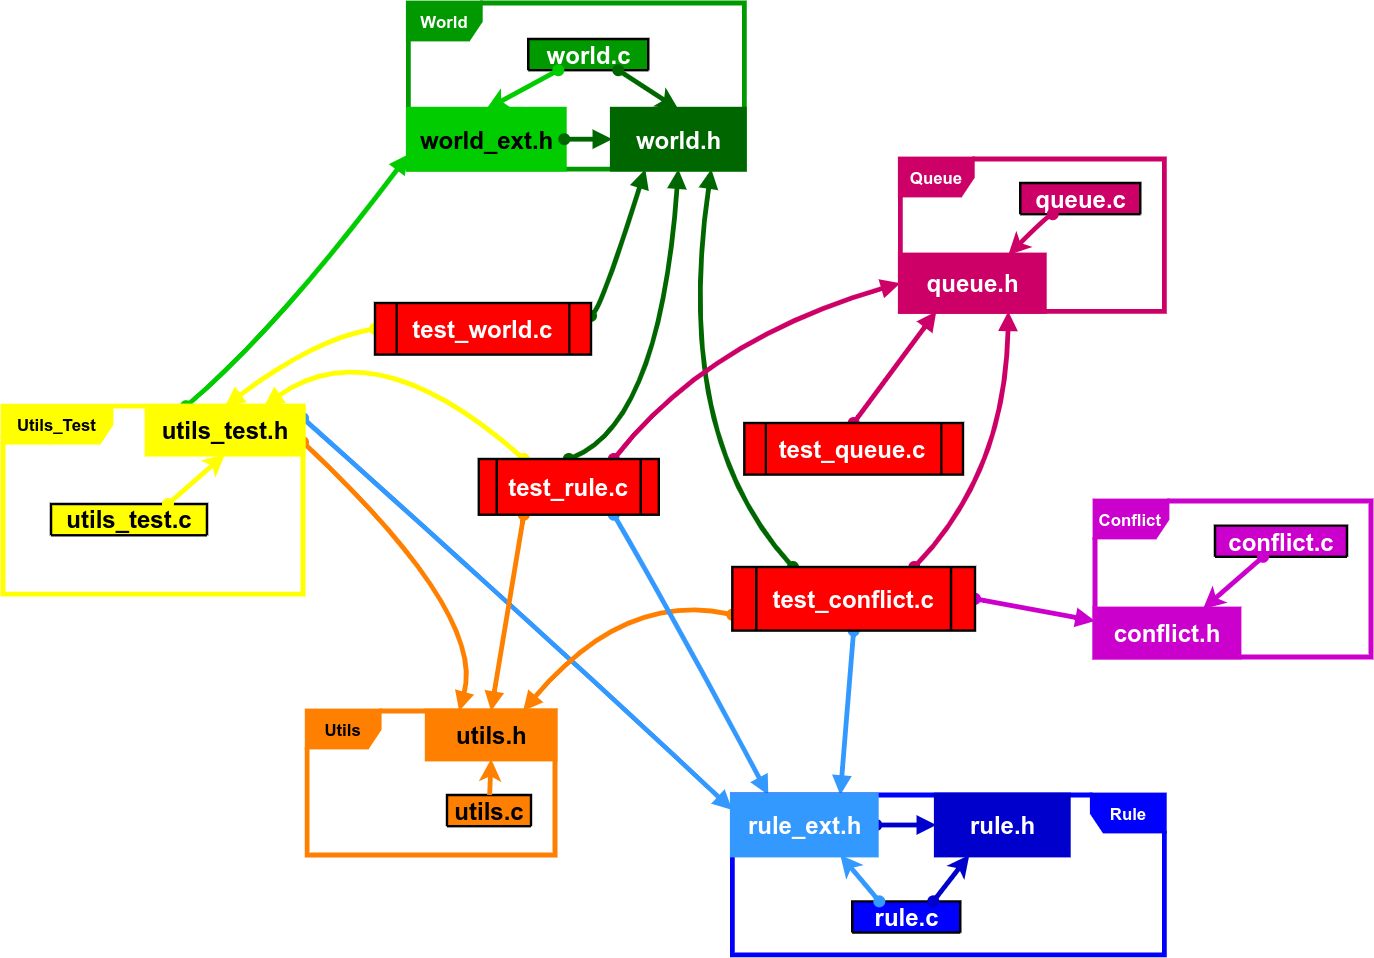
\includegraphics[width=\textwidth]{tst.png}
        \caption{Dépendances des tests}
        \label{fig:GrapheDepTests}
    \end{subfigure}
    \caption{Graphes des dépendances du projet}
    \label{fig:GrapheDep}
\end{figure}

\chapter{Monde et ses règles}
\section{Représentation et fonctionnement d'un monde}
\subsection{Définition d'un monde}
La structure du monde est imposé par le sujet : un tableau de dimension $\texttt{WIDTH} \times \texttt{HEIGHT}$. Il est constitué de nombres entiers positifs compris entre $0$ et $4294967295$ \footnote{Cet entier est la valeur maximale que peut prendre un entier positif (\lstinline{max unsigned_int}) en C} représentant l'état d'une cellule. A chaque élément du tableau est associé une couleur, également appelé état. Il existe une bijection entre le tableau d'un monde et sa représentation 2D comme on peut le voir sur la \autoref{fig:Conv_array_2D}. On a donc la relation suivante : $$i* WIDTH + j = k ,$$ k étant l'indice dans le tableau et $(i,j)$ les indices dans le monde 2D.

\begin{figure}[ht!]
    \centering
    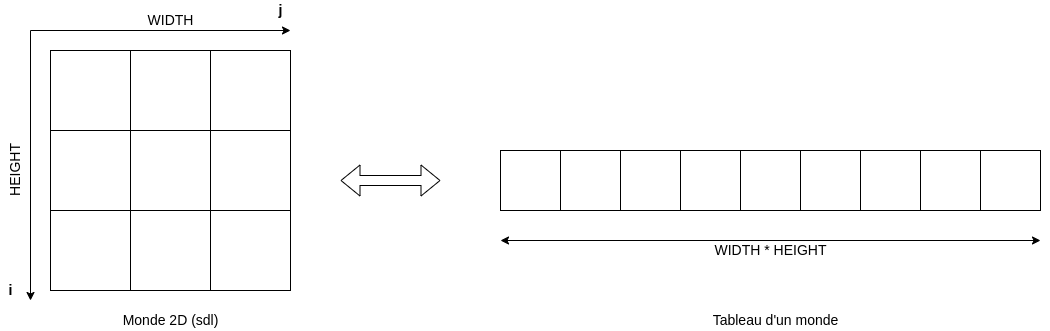
\includegraphics[width=0.95\textwidth]{"chap2/2D_to_Array.png"}
    \caption{Relation entre un tableau à une image de taille $\texttt{WIDTH}\times\texttt{HEIGHT}$}
    \label{fig:Conv_array_2D}
\end{figure}

Le monde est considéré comme un espace torique, c'est-à-dire que lorsqu'une cellule se déplace sur les bords de l'image, à l'image d'un planisphère \footnote{Les auteurs de ce rapport se sont essayés à l'antanaclase, ils espèrent avoir correctement appréhender le concept derrière cette figure de style}, la cellule se retrouve sur le bord opposé. Pour ce faire il a fallu implémenter une fonction \lstinline{int modulo(int x, int n)} complémentaire qui prenne en compte les nombres négatifs et qui retourne dans tous les cas un nombre positif.
\begin{lstlisting}
int modulo(int x, int n)
{
    if (x < 0) {
        return n + (x % n);
    } else
        return x % n;
}
\end{lstlisting}

Pour faire le lien entre la représentation sous forme de tableau d'un monde et sa représentation 2D, nous avons implémenté la fonction \lstinline{world_disp(struct world* w)}. Il a été nécessaire que le retour sur la sortie standard de la fonction soit compatible avec la librairie \texttt{sdl} afin de pouvoir afficher en couleur l'image (voir \autoref{fig:WorldDisplay}

\begin{figure}[ht]
    \centering
    \hspace*{\fill}
    \begin{subfigure}{0.15\textwidth}
        \centering
        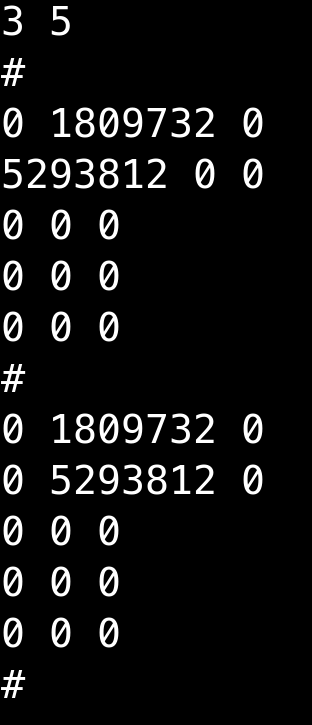
\includegraphics[width=\textwidth]{img/chap2/SortieStandard.png}
        \subcaption{Sortie Standard}
    \end{subfigure}
    \hfill
    \begin{subfigure}{0.15\textwidth}
        \centering
        
\includegraphics[width=\textwidth]{img/chap3/TestConflict1.png}
        \subcaption{Première image générée}
    \end{subfigure}
    \hfill
    \begin{subfigure}{0.15\textwidth}
        \centering
        
\includegraphics[width=\textwidth]{img/chap3/TestConflict2.png}
        \subcaption{Deuxième image générée}
    \end{subfigure}
    \hspace*{\fill}
    \caption{Sortie de \texttt{world\_display()} et résultat à l'affichage}
    \label{fig:WorldDisplay}
\end{figure}

\newpage
\subsection{Deux implémentations de monde}
\label{sec:ImplementationMonde}
Nous avons utilisé deux grandes catégories de mondes  lors de ce projet :
\begin{itemize}
    \item le monde du jeu de la vie (d'abord en noir et blanc puis en couleur) qui est généré de manière aléatoire (voir la \autoref{fig:jeu_de_la_vie});
    \item le monde du tas de sable représenté par la \autoref{fig:sablier}, (qui peut être ou ne pas être aléatoire).
\end{itemize}
\vspace{\parskip}

\begin{figure}[ht]
    \centering
    \hspace{\fill}
    \begin{subfigure}{0.35\textwidth}
        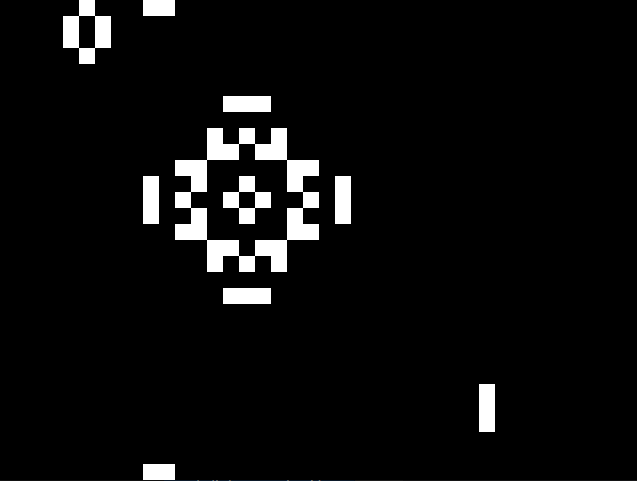
\includegraphics[width=\textwidth]{"chap2/jeu_de_la_vie.png"}
        \subcaption{Jeu de la vie}
        \label{fig:jeu_de_la_vie}
    \end{subfigure}
    \hfill
    \begin{subfigure}{0.35\textwidth}
        
\includegraphics[width=\textwidth]{chap2/sablier.png}
        \subcaption{Sablier}
        \label{fig:sablier}
    \end{subfigure}
    \hspace{\fill}
    \caption{Image obtenue avec \texttt{SDL}}
    \label{fig:sdl_mondes}
\end{figure}

L'implémentation de ces deux mondes a mis en évidence deux types de comportements pour une cellule : le changement d'état lié à son entourage (jeu de la vie) et le déplacement d'une particule (sablier).

Nous avons regroupé les quelques couleurs primaires utilisées dans ce projet dans une énumération \lstinline{enum state}. Une couleur spéciale a été réservée sous le nom de \texttt{RANDOM\_COLOR} et à l'image de la carte \og 4 couleurs \fg{} dans un jeu de UNO, correspond de manière arbitraire à toutes les couleurs à la fois. Son utilisation est abordée plus en détaille dans la \autoref{sec:ReglesMotif}.

%Ces deux mondes ont utilisé des couleurs regroupées dans une structure appelée \texttt{state} : \texttt{DEAD} (noir), \texttt{ALIVE} (blanc), \texttt{EMPTY} (bleu), \texttt{GRASS} (vert), \texttt{SAND} (jaune) et une couleur spéciale appelée \texttt{RANDOM\_COLOR}.

Afin de générer un monde initial, nous avons utilisé une fonction \lstinline{struct world world_init(char opt, int seed)}. Comme explicité plutôt, il doit est possible de générer un monde aléatoire. Pour ce faire, lors du lancement de l'exécutable principal \texttt{project}, il est nécessaire d'ajouter l'option -s (option programmable grâce à la libairie \texttt{optget}) et d'ajouter à la suite un entier qui sera une graine à la génération pseudo-aléatoire du monde.

Une dernière fonction est disponible concernant les mondes, la fonction \lstinline{void world_apply_rule()} (manque ici les paramètres, pour des raisons visuelles). Elle permet d'appliquer les règles sur les cellules lorsque nécessaire. Cette fonction étant fortement liée à la façon dont nous résolvons les conflits, on en parle plus en détail dans la \autoref{sec:Conflits}.

Finalement, lors de la génération du monde, il est important de définir ce qu'est une cellule vide. En effet, toujours lors de la gestion des conflits, nous avons fait le choix de ne déplacer une cellule que lorsque l'endroit où elle veut se déplacer est vide. Or tout état est en réalité un entier. Nous avons fait le choix de prendre la valeur 0 pour définir une cellule vide, ce qui correspond à la valeur \texttt{DEAD} dans l'énumération de nos états.

\subsection{Tests concernant les mondes et complexité des fonctions} \label{sec:ReglesMotif}

On teste la génération d'un monde aléatoire, c'est-à-dire qu'on regarde si deux mondes généré aléatoirement sont bien différents. Pour ce faire, comme il y a une petite chance que deux mondes aléatoires soient identiques, on laisse la possibilité de régénéré un monde dix fois avec la même graine. Si au cours des 1O itérations, le premier monde est identique aux 10 autres avec des graines différentes, alors on considère que la génération d'un monde aléatoire n'est pas respectée.

La fonction \lstinline{void world_apply_rule()} étant intrinsèquement liée à la gestion des conflits et à de nombreux autres paramètres externes, elle est en réalité testée dans le fichier \texttt{test\_conflict.c}.

En ce qui concerne la complexité, si on pose $W$ la longueur et $H$ la largeur de l'image, on a:
\begin{itemize}
    \item \lstinline{world_display}: on parcourt toutes les cases du monde et on les affiches donc la complexité est en $O(W\times H)$
    \item \lstinline{world_init}: la complexité est de $O(W\times H)$ (car il faut associer à chaque cellule une valeur)
\end{itemize}

\section{Implémentation et évolution des règles par motifs}

Le principe d'un automate cellulaire est de définir des règles plus ou moins compliquées au début de l'algorithme et de les appliquer sur toutes les cellules du monde. Mais comment définir une règle ?

Une règle ne s'applique sur un pixel que dans des conditions spécifiques pré-établies. Nous nous sommes donc posez la question des cellules à observer, des conditions à remplir pour que la règle s'applique. Or dans le jeu de la vie, en plus de regarder l'état de la cellule à modifier, il faut également regarder ses cellules voisines. C'est pourquoi la première  implémentation des règles repose sur les informations suivantes :
\begin{itemize}
    \item un tableau de taille 9 (\lstinline{NB_NEIGHBOUR}) contenant tous les voisins et la cellule a étudiée (située à l'indice 4 du tableau)
    \item un tableau qui contient les différentes modifications possibles (changements d'état ou déplacements) si la règle correspond à la situation du monde (la taille de ce tableau est déterminé par la valeur \lstinline{MAX_STATE}) ;
    \item le nombre de changements possibles pour une règle
\end{itemize}
\vspace{\parskip}

Par soucis de clarté, nous avons fait le choix d'implémenter les changements à appliquer par une structure qui comprend:
\begin{itemize}
    \item la valeur de la cellule
    \item le déplacement selon \texttt{dx} et \texttt{dy}
\end{itemize}

Cette structure est la suivante dans notre code :
\begin{lstlisting}
    struct next_state {
        unsigned int next_color;
        int dx, dy;
    };
\end{lstlisting}
\vspace{\parskip}

\begin{figure}[h!]
    \centering
    \begin{subfigure}{0.75\textwidth}
        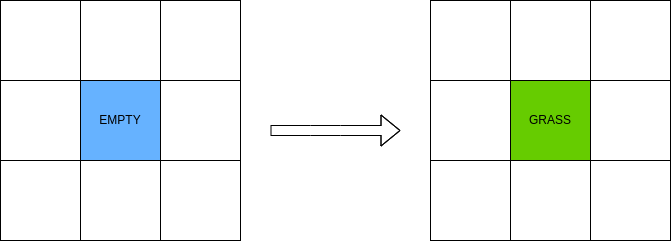
\includegraphics[width=\textwidth]{"chap2/change_couleur.png"}
        \subcaption{Changement de couleurs}
        \label{fig:chgt_color}
        \bigskip
    \end{subfigure}

    \begin{subfigure}{0.75\textwidth}
        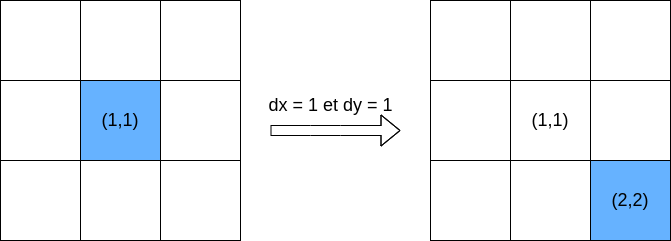
\includegraphics[width=\textwidth]{img/chap2/change_mov.png}
        \subcaption{Déplacement d'une particule}
        \label{fig:chgt_move}
    \end{subfigure}
    \caption{Les deux types de modifications pour une règle}
    \label{fig:modif_types}
\end{figure}

Nous avons choisi la convention suivante en ce qui concerne les changements d'une règle : soit on applique un déplacement, soit on applique un changement d'état. Le but de cette convention est de rester cohérent avec le principe de \bsc{Lavoisier} \footnote{En réalité, dans le jeu de la vie, des cellules naissent ou meurent, c-à-d des cellules apparaissent et disparaissent. Le principe physique précédent n'est donc pas respecté. Pour être plus juste, le principe de \bsc{Lavoisier} s'applique uniquement lorsqu'une cellule se déplace} - \emph{rien ne se perd, rien de ne crée, tout se transforme}. En effet, déplacer et modifier la couleur d'une cellule entre deux générations d'images revient à la faire disparaître.

Pour générer les règles de la vie, il a donc fallu générer tous les motifs possibles pour 9 voisins soit $2^9 = 512$ combinaisons. Nous nous sommes inspirés de l'écriture binaire pour générer tous les motifs en noir est blanc. L'inconvénient de cette méthode est qu'il correspond à la formule suivante: $$\texttt{nombre\_couleurs}^\texttt{nombre\_voisins} $$
En effet, plus le monde comporte d'états (ie plus il y a de couleurs), plus le nombre de motifs à générer est important. Il est également nécessaire de rappeler que la complexité de l'algorithme principal pour la génération d'une image dépend fortement du nombre de règles. En effet, pour chaque cellule l'algorithme cherche une règle compatible parmi toutes les règles existantes.

Une solution a été de faire des groupes de motifs en utilisant une couleur qui correspond à toutes les autres appelée \texttt{RANDOM\_COLOR} (définit dans la \autoref{sec:ImplementationMonde}). Cela à été fortement utile lors de l'implémentation de la chute de sable. Cependant, cette solution a un inconvénient. Lorsqu'on génère un motif on sait qu'il est unique. Cependant, plusieurs motifs avec des règles différentes peuvent être malencontreusement regroupés sous un même motif comportant \texttt{RANDOM\_COLOR}. En effet, en regardant le graphe \autoref{fig:motifs_avec_random}, si les cases blanches représentent cette couleur bonus, alors le motif 2 est un cas particulier du motif 1. En gagnant en complexité en diminuant le nombre de règle, on perd la bijection entre règle et motif.

\begin{figure}[ht]
    \centering
    \hspace*{\fill}
    \begin{subfigure}{0.3\textwidth}
        \centering
        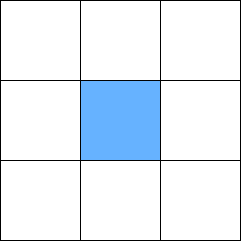
\includegraphics[width=\textwidth]{chap2/random_color1.png}
        \subcaption{Motif 1}
        \label{fig:motif2}
    \end{subfigure}
    \hfill
    \begin{subfigure}{0.3\textwidth}
        \centering
        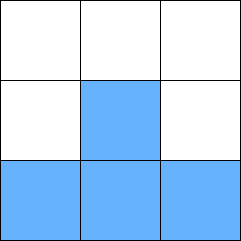
\includegraphics[width=\textwidth]{chap2/random_color2.png}
        \subcaption{Motif 2}
        \label{fig:motif1}
    \end{subfigure}
    \hspace*{\fill}
    \caption{Deux motifs : le motif (b) est inclus dans le motif (a)}
    \label{fig:motifs_avec_random}
\end{figure}

Il faut donc être prudent lors de l'implémentation des règles et de leur placement dans le tableau. En effet, c'est la première règle qui correspond qui est appliquée, les autres sont ignorées. Les règles les plus spécifiques doivent donc être en début du tableau et les plus génériques à la fin.

Cette solution n'est donc pas optimale de part sa forte complexité temporelle et sa fragilité. On doit ainsi trouver une autre manière de générer des règles, plus optimale, plus stable et surtout plus simple.

\section{Refonte des règles : des motifs aux fonctions}
\subsection{Limites des motifs}
On vient de voir que la forte complexité temporelle de la création des règles avec les motifs était un inconvénient majeur pour une bonne optimisation du projet. Mais encore, il ne semble pas intuitif d'utiliser des motifs avec certaines règles, par exemple du jeu de la vie. En effet, ce dernier ne comporte que deux règles :
\begin{itemize}
    \item Si une cellule morte est entourée par 3 cases vivantes, alors elle devient vivante
    \item Si une cellule vivante est entourée par moins d'une case vivante (isolement) ou par plus de quatre cases vivantes (surpopulation), alors elle meurt.
\end{itemize}
Il paraît donc plus naturel de chercher un moyen d'implémenter uniquement deux règles pour créer un jeu de la vie.
\subsection{Généricité des règles}
Une manière simple de représenter une règle est de le faire avec une fonction. En retournant un booléen, elle indique ainsi si elle doit être appliquée ou non. Dans l'exemple du jeu de la vie, on doit créer deux règles dans \texttt{rule.c}:
\begin{itemize}
    \item \lstinline{int born(const struct world* w, unsigned int i, unsigned int j)} pour vérifier si une cellule morte doit vivre ou pas ;
    \item \lstinline{int dead(const struct world* w, unsigned int i, unsigned int j)} pour vérifier si une cellule vivante doit mourir ou pas.
\end{itemize}

On doit alors modifier la structure d'une règle, en remplaçant le motif de la règle par un pointeur de fonction \lstinline{int (*match)(const struct world*, unsigned int, unsigned int)}, contenant dans le cadre du jeu de la vie une de ces fonctions.

La structure des règles devient alors :
\begin{lstlisting}
    struct rule {
        int (*match)(const struct world*, unsigned int, unsigned int);
        unsigned int len_changes;
        struct next_state next_state[MAX_STATE];
    };
\end{lstlisting}

Pour ce qui est des méthodes, seul la vérification de la correspondance des règles changent, puisqu'il n'est plus nécessaire de vérifier la superposition d'un motif mais simplement à exécuter la fonction pointée par l'attribut \lstinline{match} de la règle. \lstinline{rule_match()} devient alors :
\begin{lstlisting}
    int rule_match(const struct world* w, const struct rule* r, unsigned int i, unsigned int j)
    {   
        return r->match(w, i, j);
    }
\end{lstlisting}

\subsection{Avantages de la généricité des fonctions}
Améliorer les règles en passant d'une correspondance par motif à une vérification par exécution d'une fonction possède plusieurs avantages.

Le premier est la simplicité d'écriture des règles, puisqu'il est naturel de les imaginer avec une fonction. Ensuite, le cas du jeu de la vie montre qu'on obtient un gain non négligeable en espace (passage de $2^9$ à $2$ règles). En réalité, certaines règles sont plus sensibles que d'autres à ce gain. Par exemple, un monde régit par des règles de chute de sable (comme utilisé dans les \emph{achievements} 2 et 3) ne possède quasiment aucun gain avec la généricité des règles, ceux-ci étant imaginés comme pour une correspondance de motif. En revanche, une correspondance de motif reste quand même implémentable avec une fonction, ce que faisait d'ailleurs \lstinline{find_neighbours()} et \lstinline{compare_pattern ()}dans \lstinline{rule_match}.

Enfin, on réalise que l'utilisation d'une structure abstraite dans l'en-tête facilite grandement cette transition, puisqu'il a été aisé de faire cette transition sans devoir modifier le projet principal.

\chapter{Changements entre deux mondes}
\graphicspath{{img/chap3}}
Après avoir implémenté le monde et les règles, il faut maintenant mettre en place une stratégie d'applications de ces changements sur le monde. 
\section{File d'attente des changements}
Une méthode possible pour stocker les changements à effectuer entre deux monde est d'utiliser une file, qui sera alors défilé au besoin. Cette méthode permet de ne stocker que les changements réels à appliquer tout en conservant leur ordre d'application grâce à la structure en file.

\subsection{Représentation d'un changement par un nœud}
Avant même de travailler sur la file de changements, il faut dans un premier temps concevoir et implémenter un élément (un changement) de cette file.

Nous avons fait le choix de modéliser un changement à effectuer par un nœud de liste simplement chaînée, comportant les attributs suivants :
\begin{itemize}
    \item les coordonnées de la case à modifier;
    \item le numéro de la règle à appliquer;
    \item l'indice de l'état à appliquer à cette case;
    \item un pointeur vers un autre nœud : le nœud suivant dans la file.
\end{itemize}

En C, l'implémentation d'un tel objet se fait à l'aide de la structure suivante :
\begin{lstlisting}
struct change {
    unsigned int i, j, idx_rule, idx_next_state;
    struct change* next;
};
\end{lstlisting}
\label{lst:StructureChangement}
Cette structure est incorporée tel quel dans l'en-tête \texttt{queue.h} afin de rendre ses attributs accessibles aux autres parties du programme. Cela permet de récupérer et appliquer aisément la règle et l'état du changement.

\subsection{Structure de la file en liste chaînée}
Maintenant que l'on a modélisé les changements sous forme de nœuds, il nous suffit de les chaîner pour obtenir une liste chaînée de nœuds, que l'on pourra manipuler selon le fonctionnement d'une file.

Cette file est implémentée sous forme d'une structure avec les attributs suivants :
\begin{itemize}
    \item un tableau de changements, qui constitue l'espace de stockage des nœuds de la file;
    \item le nombre d'éléments de cette liste;
    \item le pointeur vers le premier nœud de la file des changements en attente;
    \item le pointeur vers le dernier nœud des changements en attente;
    \item le pointeur vers le premier nœud de la liste chaînée des changements déjà effectués.
\end{itemize}

Ceci donne en C l'implémentation suivante :
\begin{lstlisting}
struct queue {
    unsigned int len_list_changes;
    struct change list_changes[MAX_QUEUE_SIZE];
    struct change* first_to_do;
    struct change* first_done;
    struct change* last_to_do;
};
\end{lstlisting}
\label{lst:StructureQueue}
\clearpage
Cette file était dans un premier temps déclarée entièrement dans le \texttt{queue.h}, comme l'est la structure des changements. Cependant, afin de préserver les attributs de la file, nous avons décidé de déclarer uniquement une structure abstraite \lstinline{struct queue} dans l'en-tête \texttt{queue.h}, à l'image des règles. On ne travaille qu'avec une seule file \lstinline{struct queue queue} déclarée comme variable globale dans le code source de la file \texttt{queue.c}.

En plus de la file souhaitée, cette structure comporte une liste chaînée des changements déjà effectués. Celle-ci fait ainsi office de \og corbeille \fg{} de changements, sur lequel on peut éventuellement opérer et permet de \og  supprimer \fg{} un défilement sans devoir libérer un espace du tableau des changements de la file par allocation dynamique.

\subsection{Manipulation et optimisation de la file}
Une fois la structure de la file établie, il ne reste plus qu'à définir les méthodes permettant de manipuler la file.
Pour cela, on définit trois méthodes principales :
\begin{itemize}
    \item \lstinline{void queue_init()} pour initialiser une file déjà crée;
    \item \lstinline{int queue_is_not_empty()} qui indique si la file comporte un élément ou pas;
    \item \lstinline{void queue_append(unsigned int i, unsigned int j, unsigned int idx_rule, unsigned int idx_next_state)} pour ajouter un changement en queue d'une file existante;
    \item \lstinline{struct change* queue_pop()} pour récupérer le changement en tête de file et le supprimer de celle-ci.
\end{itemize}

Il est aussi utilisé deux fonctions supplémentaires :
\begin{itemize}
    \item \lstinline{create_change()}, utilisée par \lstinline{queue_append()} pour (dans une première version) ajouter simplement un changement dans le tableau et en définir les attributs du changement souhaité.
    \item \lstinline{queue_is_not_empty()} qui indique si une file est vide ou non.
\end{itemize}

L'initialisation d'une file se fait simplement en mettant à zéro le nombre de ses éléments et en mettant tous ses pointeurs à \lstinline{NULL}, ce qui permet de réinitialiser la file à chaque nouvelle image sans devoir effacer le contenu du tableau \lstinline{list_changes}. 

L'ajout d'un changement à la file se faisait dans un premier temps uniquement en éditant l'élément \lstinline{list_change[len_list_changes]} (comme décrit dans la \autoref{fig:QueueAppend}). Cependant, cette stratégie d'apparence simple pose rapidement des problème au niveau du tableau \lstinline{list_changes}, qui peut rapidement déborder et provoquer des erreurs de segmentations. Pour palier à cet inconvénient autrement qu'en agrandissant arbitrairement \lstinline{MAX_QUEUE_SIZE} = \lstinline{WIDTH*HEIGHT}, on réécrit les nouveaux changements en suivant la liste chaînée \og corbeille \fg{} \lstinline{first-done} dès que celle-ci possède un élément (voir \autoref{fig:QueueRemoveAfterAppend}). Ceci résout les problèmes d'espace mémoire sans augmenter la taille du tableau des changements tant qu'on opère bien un seul changement par cellule du monde, ce qui est bien le cas dans le programme principal.

\begin{figure}[ht]
\centering
\begin{subfigure}{0.45\textwidth}
    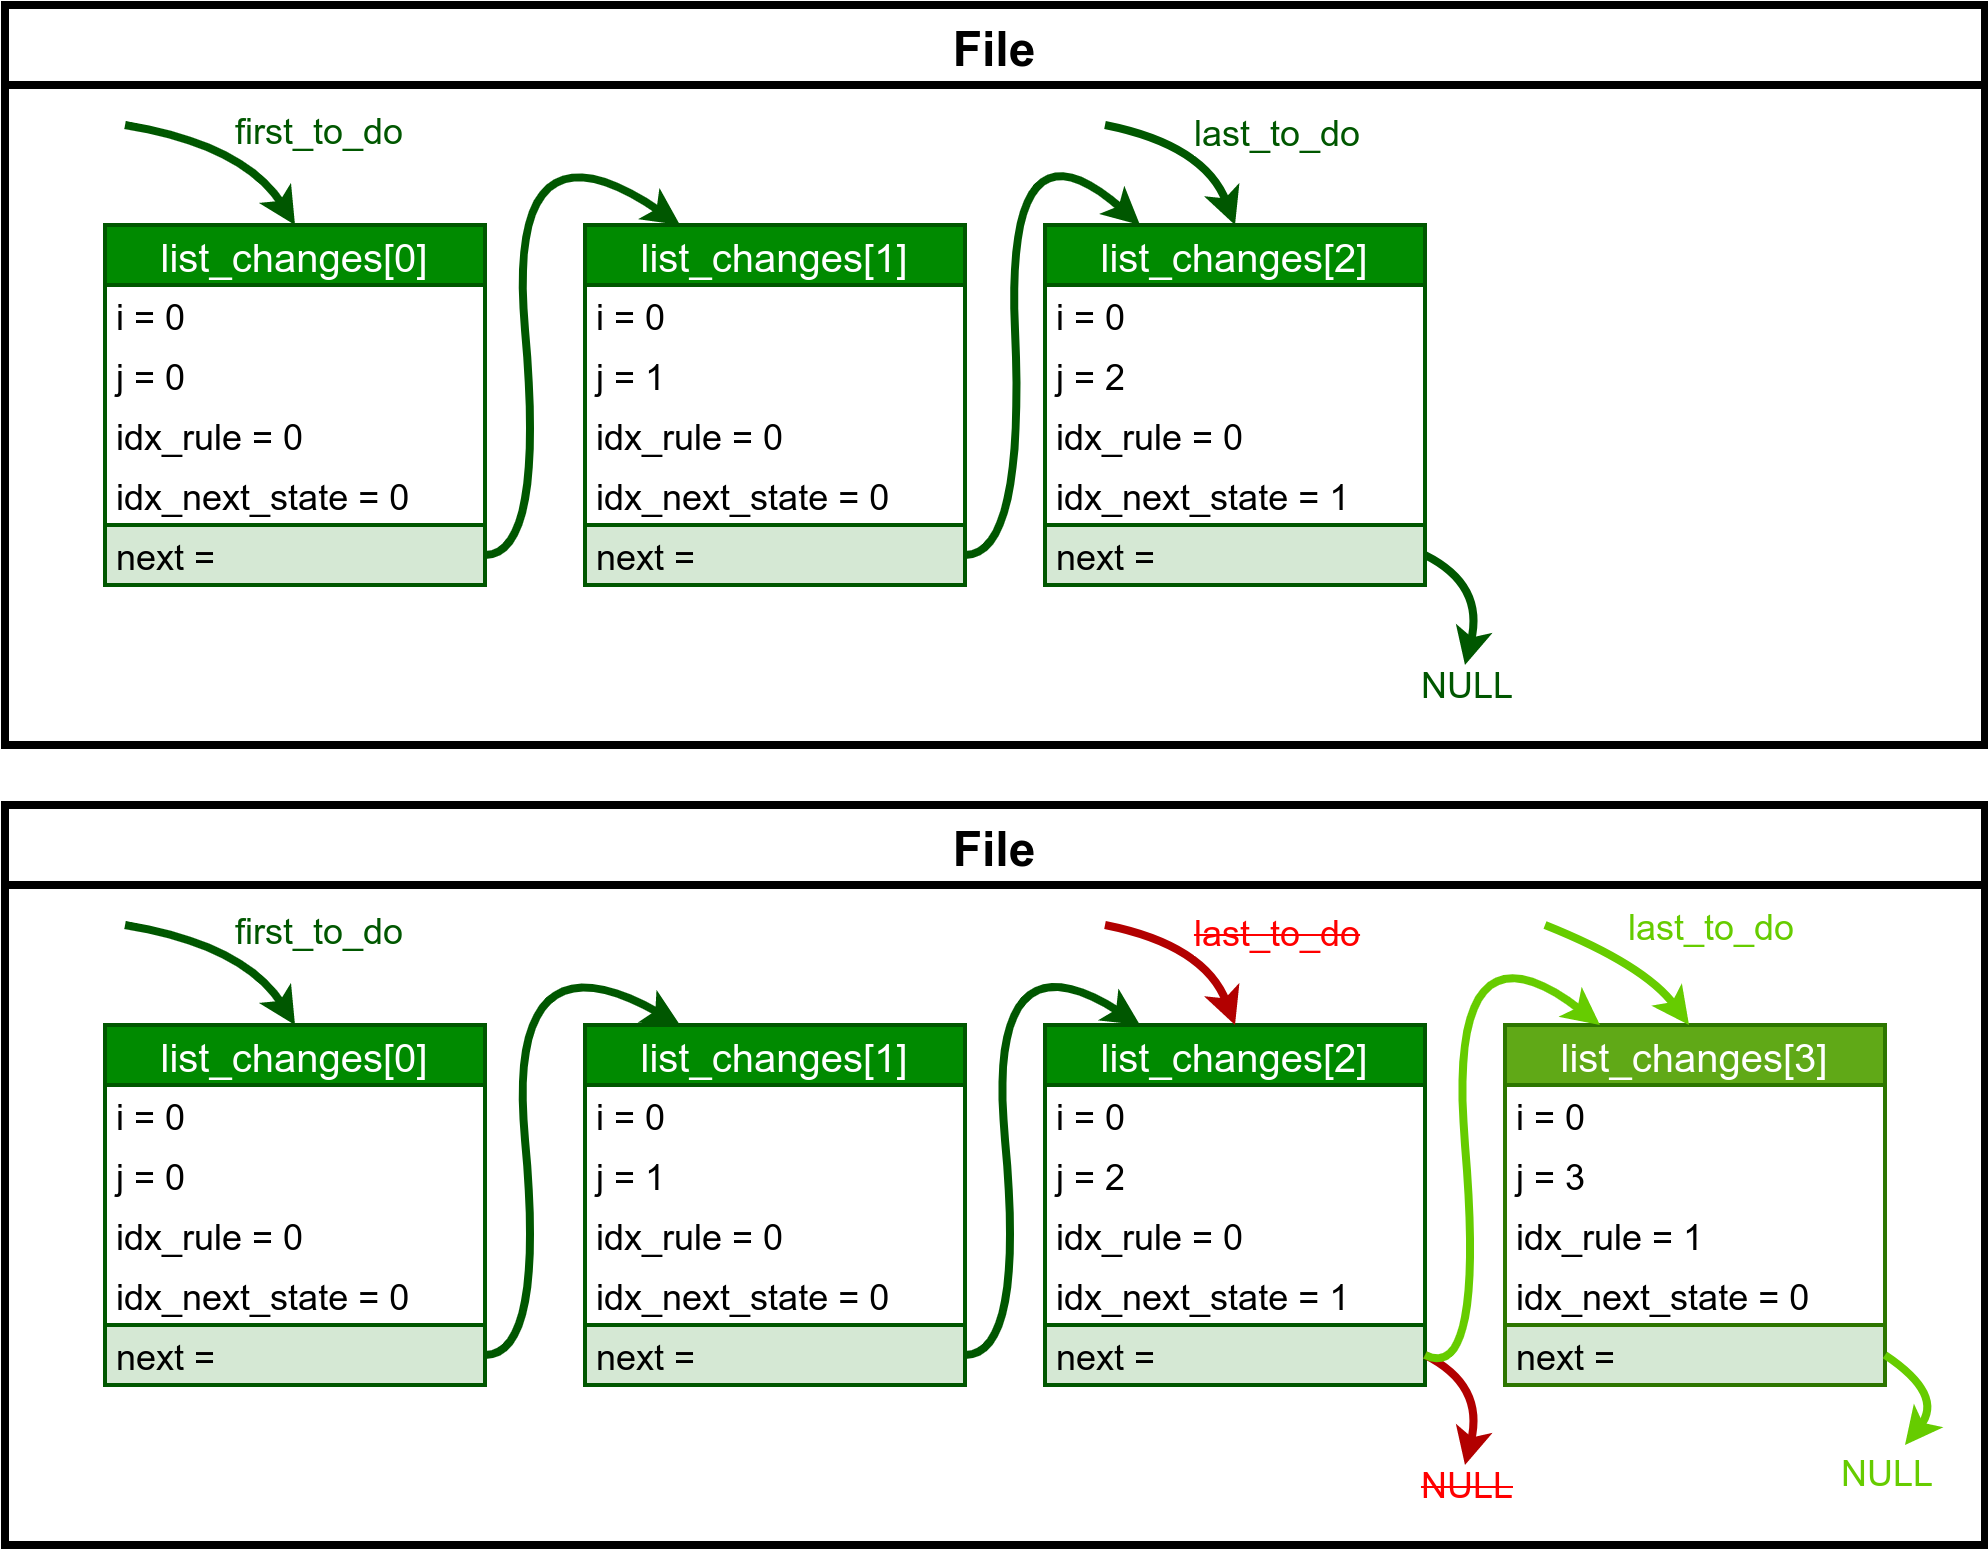
\includegraphics[width=\textwidth]{queue_append.png}
    \subcaption{Ajout d'un élément à la file}
    \label{fig:QueueAppend}
\end{subfigure}
\hfill
\begin{subfigure}{0.45\textwidth}
    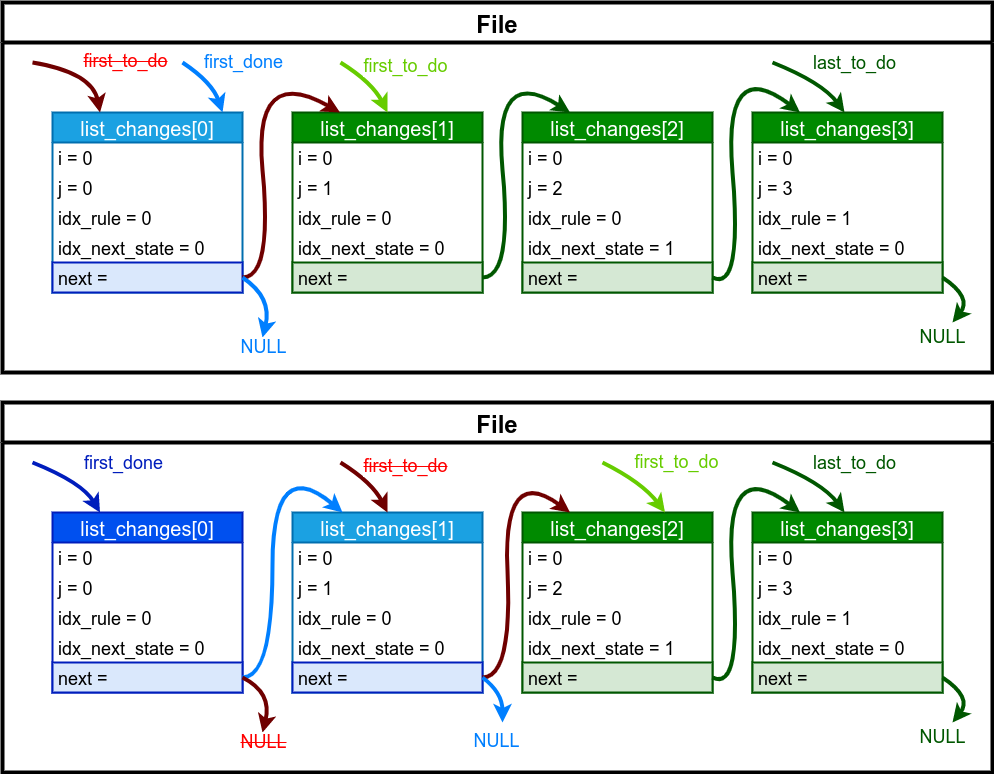
\includegraphics[width=\textwidth]{queue_pop.png}
    \subcaption{Suppression d'un élément de la file}
    \label{fig:QueueRemove}
\end{subfigure}
    \caption{Fonctionnement interne de la file}
    \label{fig:Queue}
\end{figure}

\clearpage
\begin{figure}[h!]
\ContinuedFloat
    \centering
    \begin{subfigure}{0.45\textwidth}
        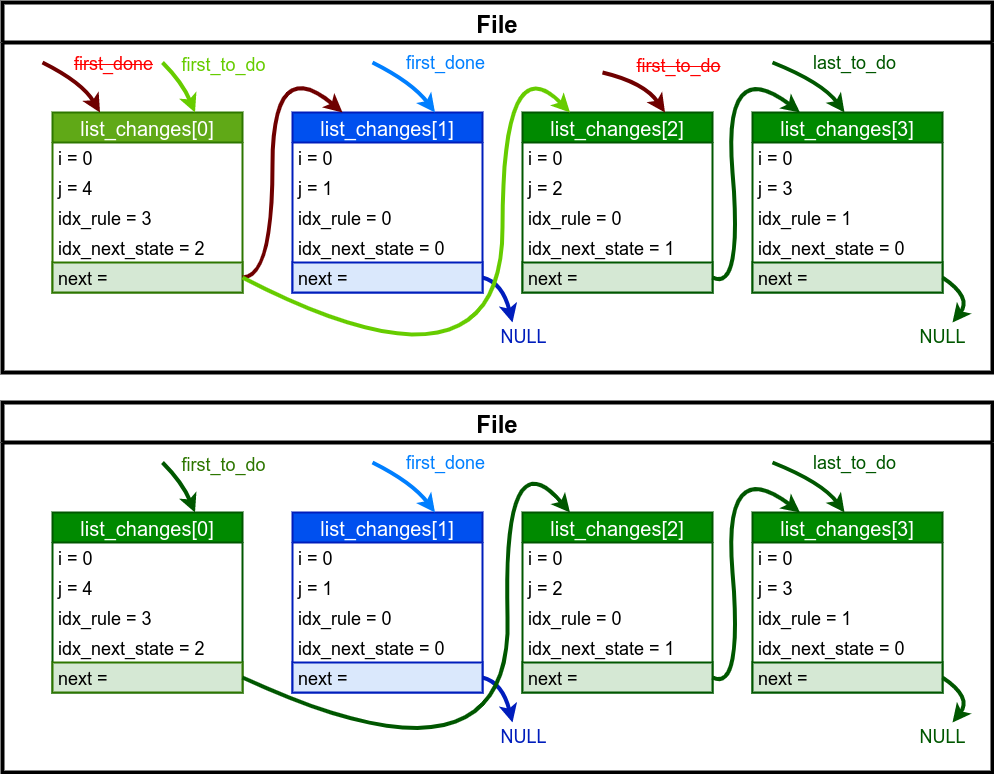
\includegraphics[width=\textwidth]{queue_popAfterAppend.png}
        \subcaption{Ajout d'un élément après une suppression (après optimisation)}
        \label{fig:QueueRemoveAfterAppend}
    \end{subfigure}
    \caption{Fonctionnement interne de la file (suite)}
\end{figure}

\subsection{Correction et complexités de la file}
Pour vérifier le bon comportement de la file, nous avons créé l'exécutable \texttt{test\_queue} (intégré aux tests exécutés par \texttt{makefile test}. Celui-ci permet de tester le bon fonctionnement des méthodes de la file, c'est-à-dire l'ajout, la suppression d'un changement et l'existence d'un élément dans la file ou non.. À chaque fois, on vérifie le bon nombre d'éléments et on vérifie leur bon emplacement dans l'espace mémoire, par un test et un affichage sur la sortie standard par les fonctions \lstinline{void queue_view_to_do()} et \lstinline{void change_view(struct change* change)}.

D'après ce qu'on a vu précédemment, la complexité temporelle des différentes fonctions de manipulations de la file sont constantes, puisqu'elles ne sont constituées que d'un nombre constant de manipulations de pointeurs. De même, la complexité en espace de la file ne sera caractérisée que par l'espace pris par le stockage des changements par \lstinline{list_changes}, qui est égale à la taille du monde.

En définitive, l'utilisation de cette file est de complexité temporelle constante et cette dernière possède une complexité spatiale linéaire en la taille du monde.

\section{Gestion des conflits}
On a vu précédemment que l'on parcourt chaque cellule d'un monde à chaque image pour estimer s'il y a un changement à effectuer ou pas. Cependant, dès que l'on inclut un déplacement de cases dans les règles, il peut arriver que deux cases veulent aller au même endroit à l'image suivante, ce qui pose problème. Ces situations constituent des conflits, que l'on doit gérer.

\subsection{Marquage d'un conflit}
Gérer un conflit commence d'abord par le détecter. Pour cela, on utilise un tableau de la taille du monde qui stocke le nombre de cellules qui souhaitent se déplacer vers une autre. On conserve également le nombre de conflits restant à gérer. Un conflit est ainsi implémentée en C par la structure suivante :
\begin{lstlisting}
struct conflict {
    unsigned int nb_conflicts;          //Nombre de cellules devant aller à celle-ci
    unsigned int conflict_to_process;   //Nombre de conflits à gérer/appliquer
};
\end{lstlisting}

Marquer l'ensemble des conflits d'un monde revient alors à créer un tableau de \lstinline{struct conflict}

Ensuite, il suffit d'incrémenter ces valeurs dès qu'une case doit se déplacer sur une cellule vide. Si la case d'arrivée n'est pas vide, la particule ne peut pas se déplacer, il n'y a donc pas de conflit. On obtient alors la détection des conflits suivante, au sein même de \texttt{project.c}~:
\begin{lstlisting}
if ((w.t[index_tmp] == EMPTY && (dx_tmp || dy_tmp)) || (!(dx_tmp || dy_tmp)) {
    t_conflicts[index_tmp].nb_conflicts += 1;
    t_conflicts[index_tmp].conflict_to_process += 1;
    queue_append(k, l, j, idx_change);
} else {
    fprintf(stderr, "Conflit perdant en %d %d car déplacement dans une case non vide.\n", k + dx_tmp, j = dy_tmp);
}
\end{lstlisting}
On remarque alors que l'ajout d'un changement à la file dépendant de l'état de la case d'arrivée. Si elle est vide, un changement est ajouté à la file. Si elle ne l'est pas, la cellule de départ reste inchangée. Ceci constitue donc déjà un début de résolution de conflit.

\subsection{Résolution des conflits} \label{sec:Conflits}
Un fois les conflits sauvegardés, on les résout au moment de vider la file et d'appliquer les changements.

Pour cela, on regarde pour chaque changement combien de conflits concerne la case où doit s'appliquer le changement :
\begin{itemize}
    \item Si la case n'a pas de conflit, alors on n'applique pas le changement, la cellule ayant déjà été modifiée ;
    \item Si la case ne comporte qu'une seule cellule voulant s'installer là, il n'y a pas de conflit et alors le changement est appliqué ;
    \item Si la case comporte plus d'une cellule voulant se déplacer là, alors on effectue un tirage au sort (suivant une loi uniforme ; $\frac{1}{\texttt{nb\_conflict}}$) pour appliquer ou non le changement :
    \begin{itemize}
    \item Si le tirage est gagné, alors la cellule est marquée comme n'ayant plus de conflit et on on applique le changement ;
    \item Sinon, la case est marquée comme ayant une cellule en moins à gérer et on n'applique pas le changement.
    \end{itemize}
\end{itemize}
Dans notre programme, c'est la fonction \lstinline{solve_conflict()} qui conditionne l'application d'un changement par \lstinline{world_apply_rule()} :
\begin{lstlisting}
int solve_conflict(struct conflict t_conflicts[], unsigned int i, unsigned int j)
{
    struct conflict c = t_conflicts[i * WIDTH + j];
    int random = rand();
    if (c.nb_conflicts == 0) { //conflit déjà résolu
        return 0;
        fprintf(stderr, "Conflit perdant en %d %d car nb_conflicts =0\n", i, j);
    } else if (c.conflict_to_process == 1) { // conflit à résoudre avec ce changement
        return 1;
    } else if ((random % c.nb_conflicts) == 0) { // changement gagnant
        t_conflicts[i * WIDTH + j].nb_conflicts = 0;
        return 1;
    } else { // changement perdant
        t_conflicts[i * WIDTH + j].conflict_to_process -= 1;
        return 0;
    }
}
\end{lstlisting}
Enfin, il suffit d'appliquer le conflit si \lstinline{solve_conflict} retourne 1. Pour cela, on change la cellule de destination selon le changement à appliquer et on rend la cellule de départ vide s'il y a eu un déplacement. La fonction \lstinline{world_apply_rule} devient alors :

\clearpage
\begin{lstlisting}
void world_apply_rule(struct world* w, struct rule* r, int i, int j,
    unsigned int idx_change, struct conflict t_conflicts[])
{
    unsigned int dx = rule_change_dx(r, idx_change);
    unsigned int dy = rule_change_dy(r, idx_change);
    int s = solve_conflict(t_conflicts, modulo(i + dx, HEIGHT), modulo(j + dy, WIDTH));
    if (s) { //si la résolution de conflit dit qu'on doit appliquer le changement
        if (dx || dy) { // il y a déplacement
            w->t[modulo(i + dx, HEIGHT) * WIDTH + modulo(j + dy, WIDTH)] = rule_change_to(r, idx_change);
            w->t[i * WIDTH + j] = DEAD; // la cellule de départ est vide
        } else { // changement de couleur uniquement
            w->t[i * WIDTH + j] = rule_change_to(r, idx_change);
        }
    }
}
\end{lstlisting}

\subsection{Correction et efficacité de la gestion des conflits}
La résolution des conflits se faisant de manière aléatoire, il est difficile d'automatiser les tests pour vérifier si les conflits sont biens gérés comme tel. Nous avons donc choisi de faire un test simplement \og visuel \fg{}, en recréant un monde simple mettant en situation un conflit entre deux cellules voulant aller au même endroit, de manière cyclique au fur et à mesure des images. En générant un grand nombre d'images et donc de conflits, on doit pouvoir apercevoir le caractère aléatoire de la résolution de conflit. Les résultats de ces tests sont illustrés 
\autoref{fig:TestConflict}
\begin{figure}[ht]
    \centering
    \begin{subfigure}{0.2\textwidth}
        
\includegraphics[width=\textwidth]{TestConflict1.png}
        \subcaption{Création d'un conflit entre deux cellules allant au centre}
        \label{fig:TestConflict1}
    \end{subfigure}
    \hfill
    \begin{subfigure}{0.2\textwidth}
        
\includegraphics[width=\textwidth]{TestConflict2.png}
        \subcaption{Victoire de la cellule jaune, attente de la cellule verte}
        \label{fig:TestConflict2}
    \end{subfigure}
    \hfill
    \begin{subfigure}{0.2\textwidth}
        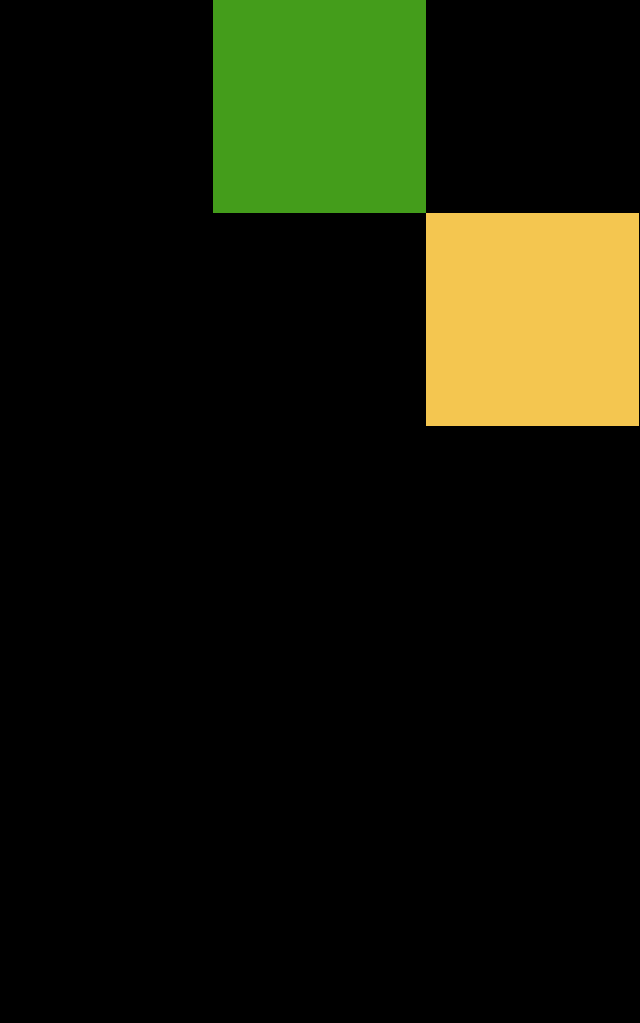
\includegraphics[width=\textwidth]{TestConflict3.png}
        \subcaption{Attente de la cellule verte car case d'arrivée non-vide}
        \label{fig:TestConflict3}
    \end{subfigure}
    \hfill
    \begin{subfigure}{0.2\textwidth}
        
\includegraphics[width=\textwidth]{TestConflict4.png}
        \subcaption{Victoire de la case verte dans la situation vu en \autoref{fig:TestConflict1}}
        \label{fig:TestConflict4}
    \end{subfigure}
    \caption{Tests de la résolution des conflits}
    \label{fig:TestConflict}
\end{figure}

Pour ce qui est de l'efficacité de la résolution des conflits, notre implémentation semble cohérente au reste de notre programme. En effet, nous ne parcourons jamais le tableau des conflits en entier (ce qui permet de garder les avantages temporaires de la file). De plus, les conflits sont stockés lors de l'ajout à la file et les conflits sont résolus lors des défilements des changement. On en déduit que la complexité spatiale de la résolution n'est uniquement impactée par le tableau de marquage des conflits, qui possède la même taille que le monde. De plus, la résolution ne nécessite aucune boucle, puisqu'elle ne fait que décider d'une application d'un changement ou non. Au final, on en déduis que la complexité de la gestion des conflits est constante en temps et linéaire en espace suivant la taille du monde.

\chapter{Conclusion}

En conclusion de ce rapport, nous souhaitons faire un bilan des apports techniques, organisationnels et humains de ce projet ainsi que des difficultés rencontrées

D'un point de vu purement technique, ce projet nous a appris l'utilisation de Git et de \texttt{make} via le \texttt{Makefile}, des outils nouveaux pour deux étudiants tout droit sortis des classes préparatoires. La gestion des conflits a été particulièrement formateur, tout comme celle de la compilation séparée aidée par le \texttt{Makefile}. Pour ce qui est de la partie programmation en elle-même, c'est la mise en pratique des connaissances vues en cours et parfois abstraites qui ont été le plus enrichissant. Savoir quand et comment utiliser des structures, des pointeurs (variables et fonctions), utiliser des librairies (\texttt{getopt}, \texttt{SDL}) afin d'optimiser au mieux nos codes sont une première expérience qui nous semble fondamental pour la consolidation de nos connaissances. On a aussi pu sentir l'aspect \og orienté objet\fg{} que proposait ce projet, notamment avec la structure abstraite des règles permettant de les modifier isolément du reste du programme. Enfin, tester notre code est aussi une compétence importante que l'on a commencé à acquérir grâce à ce projet, même si ce point nous a posé des difficultés, notamment savoir exactement quoi tester dans un code, et encore plus comment le tester. 

Mais gérer ce premier projet nous a surtout obligé a acquérir des compétences organisationnelles et humaines essentielles pour le mener à bien. Respecter les contraintes, anticiper l'évolution du code et le tester au fil de son avancement ont été des compétences à apprendre sur le tas, surtout pour une première véritable expérience de projet. Penser à commenter de manière juste et concise nos algorithmes a été une autre de nos difficultés, même si peu contraignantes dans le cadre d'un projet comme celui-ci. La répartition de notre code dans de nombreux fichiers nous a posé quelques difficultés. Cela nous a poussé à repenser l'organisation de notre code et de réaliser l'importance d'un graphe de dépendances.

Pour finir, un projet en binôme se mène à deux, et il est fondamental de gérer le travail de chacun pour ne pas se marcher dessus et rester sur la même longueur d'onde. La bonne-entente et la coopération est nécessaire et essentielle pour avancer, et nous avons eu la chance de conserver ces avantages sans qui le projet n'aurait pas été mené à bout.

\end{document}